% Copyright 2004 by Till Tantau <tantau@users.sourceforge.net>.
%
% In principle, this file can be redistributed and/or modified under
% the terms of the GNU Public License, version 2.
%
% However, this file is supposed to be a template to be modified
% for your own needs. For this reason, if you use this file as a
% template and not specifically distribute it as part of a another
% package/program, I grant the extra permission to freely copy and
% modify this file as you see fit and even to delete this copyright
% notice. 

\documentclass{beamer}

% There are many different themes available for Beamer. A comprehensive
% list with examples is given here:
% http://deic.uab.es/~iblanes/beamer_gallery/index_by_theme.html
% You can uncomment the themes below if you would like to use a different
% one:
%\usetheme{AnnArbor}
%\usetheme{Antibes}
%\usetheme{Bergen}
%\usetheme{Berkeley}
%\usetheme{Berlin}
%\usetheme{Boadilla}
%\usetheme{boxes}
%\usetheme{CambridgeUS}
%\usetheme{Copenhagen}
%\usetheme{Darmstadt}
%\usetheme{default}
%\usetheme{Frankfurt}
%\usetheme{Goettingen}
%\usetheme{Hannover}
%\usetheme{Ilmenau}
%\usetheme{JuanLesPins}
%\usetheme{Luebeck}
\usetheme{Madrid}
%\usetheme{Malmoe}
%\usetheme{Marburg}
%\usetheme{Montpellier}
%\usetheme{PaloAlto}
%\usetheme{Pittsburgh}
%\usetheme{Rochester}
%\usetheme{Singapore}
%\usetheme{Szeged}
%\usetheme{Warsaw}

\usepackage{kotex}
\usepackage{braket}
\usepackage{array}
\usepackage{calc}
\usepackage{datetime}
\usepackage{dsfont}
\usepackage{amsmath}
\usepackage{listings}


\title{Lecture 7 : 확률 }

% A subtitle is optional and this may be deleted
\subtitle{Fastcampus Math Camp}

\author{신승우}
% - Give the names in the same order as the appear in the paper.
% - Use the \inst{?} command only if the authors have different
%   affiliation.

% \institute[Universities of Somewhere and Elsewhere] % (optional, but mostly needed)
% {
  % \inst{1}%
  % Department of Computer Science\\
  % University of Somewhere
  % \and
  % \inst{2}%
  % Department of Theoretical Philosophy\\
  % University of Elsewhere}
% - Use the \inst command only if there are several affiliations.
% - Keep it simple, no one is interested in your street address.

% - Either use conference name or its abbreviation.
% - Not really informative to the audience, more for people (including
%   yourself) who are reading the slides online

\subject{Theoretical Computer Science}

% This is only inserted into the PDF information catalog. Can be left
% out. 

% If you have a file called "university-logo-filename.xxx", where xxx
% is a graphic format that can be processed by latex or pdflatex,
% resp., then you can add a logo as follows:

% \pgfdeclareimage[height=0.5cm]{university-logo}{university-logo-filename}
% \logo{\pgfuseimage{university-logo}}

% Delete this, if you do not want the table of contents to pop up at
% the beginning of each subsection:


\AtBeginSection[]
{
  \begin{frame}<beamer>{Outline}
    \tableofcontents[currentsection,hideallsubsections]
  \end{frame}
}

% Let's get started
\begin{document}

\begin{frame}
 \titlepage
\end{frame}


% \begin{frame}{선형변환의 예시 : 확대/축소} 
% 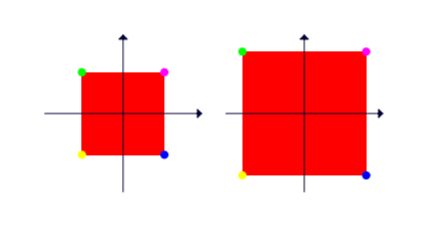
\includegraphics[width=10cm,keepaspectratio]{scale1}
% \end{frame}

% \begin{frame}{Outline}
  % \tableofcontents[hideallsubsections]
  % % You might wish to add the option [pausesections]
% \end{frame}

% Section and subsections will appear in the presentation overview
% and table of contents.


\section{확률의 정의} 

\subsection{확률의 정의}

\begin{frame}[allowframebreaks]{확률의 정의}

우리가 어떤 실험에 앞서서, 나올 수 있는 모든 가능한 결과는 알지만 그 각각 중 무엇이 나올지 모른다고 생각하자. 나올 수 있는 모든 가능한 결과의 집합을 \textbf{표본공간(Sample Space)}이라 한다. 예컨대, 

\begin{itemize} 
\item 동전을 던짐 : $S_1 = \{Head, Tail\}$
\item 주사위를 던짐 : $\{1,2,3,4,5,6\}$
\item 두 개의 동전을 던짐 : $S_1 \times S_1$
\item 0부터 1 사이의 숫자를 아무렇게나 고름 : $\{x|0 \geq x \geq 1\}$
\end{itemize}

라고 할 수 있다. 

\framebreak 

이 때, 표본공간의 부분집합을 \textbf{사건(Event)}라고 한다. 예컨대, 집합 $S_1$의 부분집합은 총 4개로, $\{\}, \{Head\}, \{Tail\}, \{Head, Tail\}$ 이다. 이 부분집합 각각을 사건이라 하며, 어떤 사건이 일어났다는 것은 관측 결과가 그 사건의 원소임을 의미한다. 예컨대, 동전을 던져서 앞면(Head)가 관측된다면, 두 이벤트 $\{Head\}, \{Head, Tail\}$이 일어난 것이다. 

만약 두 사건 E, F의 교집합이 공집합이라면, 이 때 E,F를 \textbf{배반사건(Mutually Exclusive)}라 한다. 

\framebreak

위에서 언급된 용어들을 이용하여 확률을 정의할 수 있다. 

\begin{block}{확률}
확률은 사건을 실수에 대응시키는 함수 P 중 다음 3가지 조건을 만족하는 것을 말한다. 

\begin{itemize} 
\item $\forall E \subset S, 0 \geq P(E) \geq 1$
\item P(S) = 1
\item $M = \{E_i| \forall E_i, E_j \in M,  E_i \cup E_j = \phi\}, P(\cup_{e \in M} e) = \sum_{e \in M} P(e)$
\end{itemize}
\end{block}

예컨대, 

\begin{itemize} 
\item 양수 p에 대해서 $P(\{Head\})=p$ 이고 $P(\{Tail\})=1-p$라면 P는 동전던지기 실험에 대한 확률이다. 
\item 임의의 유한한 표본공간 S에 대해서, 함수 $P(E) = \frac{|E|}{|S|}$는 항상 확률이다. 
\end{itemize}
 
\end{frame}

\subsection{조건부확률} 

\begin{frame}[allowframebreaks]{조건부확률}

내일의 날씨를 예측할 때, 전날 밤에 달무리가 관측(이 사건을 M이라 하자)되었으면   다음 날 비가 올(이 사건을 R이라 하자) 확률이 높을 것이다. 예를 들어서 다음과 같이 생각할 수 있다. 

\begin{itemize} 
\item M이 일어날 확률을 0.2라 하자. 
\item M이 일어남 $\rightarrow$ R이 일어날 확률 0.9
\item M이 일어나지 않음 $\rightarrow$ R이 일어날 확률 0.3
\end{itemize}

\framebreak

이 때, M과 R이 일어나거나, 일어나지 않을 경우에 따라서 각각 4 가지 경우를 생각할 수 있다. 이를 표를 이용하여 확률계산을 해 보자.

\begin{table}[]
\begin{tabular}{|l|l|l|l|}
\hline
      & M              & not M          & prob \\ \hline
R     & 0.2*0.9 = 0.18 & 0.8*0.3 = 0.24 & P(R) = 0.42 \\ \hline
not R & 0.2*0.1 = 0.02 & 0.8*0.7 = 0.56 & P(not R) = 0.58 \\ \hline
prob  & P(M) = 0.2     & P(not M) = 0.8            & 1    \\ \hline
\end{tabular}
\end{table}

위와 같이 계산할 수 있다. 이 때, M이 일어났을 때 R이 일어날 확률(조건부확률)과, M과 R이 같이 일어날 확률을 구분하여 생각하여야 한다. 전자의 조건은 표본집단이 M이 일어난 집단으로 바뀌고, 후자의 경우는 전체 표본집단 하에서의 확률을 생각하기 때문이다. 즉, 2행 2열의 확률은 M과 R이 같이 일어난 확률이지만, 이를 P(M)으로 나누면 0.9가 되어 원 조건을 만족하게 된다. 


\framebreak
이에서 다음의 공식을 생각할 수 있다. 

\begin{block}{조건부확률}
F가 일어났다는 선행조건 하에서 F가 일어날 확률을 P(E|F)라고 쓰며, $P(E|F) = \frac{P(E  F)}{P(F)}$ 로 계산한다. 
\end{block}

\framebreak


이 때, 조금 다른 상황을 생각해 보자. 길동이가 노란 옷을 입는 사건을 Y라고 하면, 이 때 일반적으로 길동이의 옷 색과 비가 내릴 확률은 상관이 없을 것이므로 위 상황과 같은 확률로 비가 온다고 생각하면, 다음이 성립할 것이다. 

\begin{itemize} 
\item R이 일어날 확률은 0.42, Y가 일어날 확률은 0.1
\item Y가 일어남 $\rightarrow$  R이 일어날 확률 0.42
\item Y가 일어나지 않음 $\rightarrow$ R이 일어날 확률 0.42 
\end{itemize}

\framebreak

이 때는 위와 비슷하게 아래 표를 생각할 수 있다. 

\begin{table}[]
\begin{tabular}{|l|l|l|l|}
\hline
      & Y             & not Y          & prob \\ \hline
R     & 0.1*0.42 = 0.042 & 0.9*0.42 = 0.24 & P(R) = 0.42 \\ \hline
not R & 0.9*0.58 = 0.522 & 0.1*0.58 = 0.058 & P(not R) = 0.58 \\ \hline
prob  & P(Y) = 0.1     & P(not Y) = 0.9            & 1    \\ \hline
\end{tabular}
\end{table}

즉, 이렇게 상관없는 두 사건의 경우, P(E|F) = P(E)이다. 이를 두 사건이 서로 \textbf{독립사건}이라고 한다. 이 경우, 위 식에 의해서 $P(E  F) = P(E)P(F)$이다. 


\framebreak



위 두 경우에서 일반화시켜, 사건 E와 표본공간을 분할하는 $F_i$들에 대해서 $P(E|F_i)$들이 알려져 있다고 할 때, $P(F_j|E)$를 다음과 같이 계산할 수 있다. 

이 때 분할은 다음의 두 가지를 의미한다. 

\begin{itemize} 
\item $F_i$들의 합집합이 표본공간이 된다. 
\item $F_i$끼리는 교집합이 모두 공집합이다. 
\end{itemize}


이 때, 어떤 표본공간의 부분집합 E에 대해서 다음이 성립한다. 

\begin{eqnarray} 
P(E) &=& \cup P(EF_j) \\ 
P(E) &=& \sum P(EF_j) \\ 
&=& \sum P(E|F_j)P(F_j)
\end{eqnarray}

\framebreak

또한, 어떤 특정한 $F_j$에 대해서 

\begin{equation} 
P(F_j|E) = \frac{P(EF_j)}{P(E)}
\end{equation}

이므로, 다음이 성립한다. 

\begin{equation} 
P(F_j|E) = \frac{P(EF_j)}{ \sum P(E|F_j)P(F_j)}
\end{equation}

이를 베이즈의 정리라고 한다. 

\end{frame}





\section{확률변수} 


\subsection{확률변수의 정의} 
 
\begin{frame}{Motivation}
실험 값 자체가 중요한 경우도 있지만, 가끔은 실험 값을 가공한 결과값이 더 중요할 때가 있다. 예컨대, 주사위 두 개를 던져서 그 합의 짝/홀로 승패르 가르는 게임을 한다고 하면, 주사위 각각의 결과값은 크게 중요하지 않을 것이다. 

이런 결과값은 수학적으로 볼 때, 표본공간의 각 원소들에 대한 함수라고 볼 수 있다. 이런 함수를 \textbf{확률변수(Random Variable)}이라고 한다. 
\end{frame}
 

\begin{frame}[allowframebreaks]{확률변수}

\begin{block}{확률변수}
표본공간을 정의역으로, 실수를 공역으로 가지는 \textbf{함수}를 그 표본공간에서의 확률변수라고 한다. 
\end{block}

확률변수의 예시로, 동전을 앞면이 나올 때까지 던지는 횟수를 생각하자. 그러면, 표본공간 S와 확률변수 N은 다음과 같이 정의된다. 

\begin{itemize} 
\item $S = \cup_{i=1}^n F_i$ 
\item $F_i = \{(T, T, ..., T, H)\}$ 
\item $P(F_i) = (1-p)^{i-1} p$ 
\item $N(F_i) = i$ 
\end{itemize}

이 때, p는 동전을 던져서 앞면이 나올 확률이다. 
\end{frame}

\begin{frame}{이산 확률변수}


\begin{block}{이산 확률변수(Discrete Random Variable)}
가산집합이거나 유한집합인 표본집합 위에서의 확률변수를 이산 확률변수라고 한다. 
\end{block}

이 때, 이산 확률변수 X에 대해서 

\begin{itemize} 
\item Probability Mass Function(PMF) : $f(a) = P(X=a)$
\item Cummulative Distribution Function(CDF) : $F(a) = P(X \leq a) = \sum_{x \leq a} f(a)$
\end{itemize}

가 정의된다. 이산 확률분포는 보통 PMF를 이용하여 정의된다. 예컨대, 앞장에서의 동전을 던지는 실험을 보면, $f(i) = (1-p)^{i-1}p$가 pmf이다. 이 때, 정의역 구간 내에서 pmf의 합은 1이 되어야 한다. 이는 저 식으로 1부터 무한대까지 더하는 극한을 통해 알아볼 수 있다. 

위와 같이, p같은 변수를 보통 parameter이라고 부른다. 


\end{frame}

\begin{frame}[allowframebreaks]{다양한 이산 확률변수들}

\begin{itemize} 

\item 베르누이 확률변수 
\begin{block}{베르누이 확률변수} 
pmf f가 다음과 같이 주어지는 확률변수를 베르누이 확률변수라 한다. 

\begin{eqnarray} 
f(0) &=& P(X=0) = 1-p \\ 
f(1)  &=& P(X=1) = p 
\end{eqnarray}

\end{block}

이는 어떤 성공할 확률이 p인 시행이 성공하면 1, 실패하면 0인 확률변수라고 볼 수 있다. 이것이 n번 시행되는 경우를 Binomial Random Variable이라고 한다. 이 때의 pmf f는 시행횟수 n과 성공확률 p에 대해서 다음과 같다. 

\begin{equation} 
f(i) = \left( \begin{matrix} n \\ i \end{matrix} \right) p^i (1-p)^{n-i} 
\end{equation}



\item 기하학적 확률변수

\begin{block}{기하학적 확률변수}

기하학적 확률변수는 pmf f가 parameter p에 대해서 다음과 같이 주어지는 확률변수를 뜻한다. 

\begin{equation} 
f(i) = P(X=i) = (1-p)^{i-1} p
\end{equation}

\end{block}


\item 푸아송 확률변수

\begin{block}{푸아송 확률변수}
푸아송 확률변수는 pmf f가 파라미터 $\lambda$에 대해서 다음과 같이 주어지는 확률변수를 뜻한다. 

\begin{equation} 
f(i) = P(X=i) = e^{-\lambda} \frac{\lambda^i}{i!}
\end{equation}
\end{block}

\end{itemize}

\end{frame}


\begin{frame}{연속 확률변수}
\begin{block}{연속 확률변수}
비가산집합인 표본공간 하에서의 확률변수를 연속 확률변수라고 한다. 
\end{block}

연속 확률변수의 경우, P(X=a)는 언제나 0이다. 따라서 pmf와 같은 개념은 없으나, 이와 비슷한 probability distribution function(PDF)를 이용하여 정의한다. 즉, 다음을 임의의 정의역 내 부분집합 B에서 만족하는 함수 f를 pdf라 한다. 

\begin{equation} 
P(X \in B) = \int_B f(x)dx 
\end{equation}

위와 비슷하게, probability cumulative distribution F는 다음과 같이 정의된다. 

\begin{equation} 
F(a) = P(X \in (-\infty, a])) = \int^a_{-\infty} f(x)dx
\end{equation}

이 때, 위 두 식에서 $\frac{d}{dx}F(x) = f(x)$가 성립함을 알 수 있다. 
\end{frame}



\begin{frame}[allowframebreaks]{다양한 연속 확률분포} 
\begin{itemize} 

\item Uniform Random Variable 

\begin{block}{Uniform Random Variable}

Uniform Random Variable은 pdf f가 parameter (a,b)에 대해서 다음과 같이 주어지는 확률변수를 뜻한다. 

\begin{equation} 
f(x) = \frac{1}{|a-b|}, x \in (a,b)
\end{equation} 
\end{block}
\item 감마 확률변수

\begin{block}{감마 확률변수}
감마 확률변수는 pdf f가 parameter $\lambda>0, \alpha>0$에 대해서 다음과 같이 주어지는 확률변수를 뜻한다. 

\begin{equation} 
f(x) = \frac{\lambda e^{-\lambda x} (\lambda x)^{\alpha-1}}{\Gamma(\alpha)}
\end{equation} 

이 때, 

\begin{equation} 
\Gamma(\alpha) = \int^{\infty}_0 e^{-x} x^{\alpha-1} dx
\end{equation}

이다. $\alpha= 1$인 경우, 이를 exponential random variable이라고 한다. 
\end{block}



\item 정규확률변수
\begin{block}{정규확률변수}
정규확률변수는 pdf f가 parameter $\mu, \sigma$에 대해서 다음과 같이 주어지는 확률변수를 뜻한다. 

\begin{equation} 
f(x) = \frac{1}{\sqrt{2 \pi} \sigma} e^{-(\frac{(x-\mu)^2}{2 \sigma^2})}
\end{equation} 

\end{block}

\end{itemize} 
\end{frame}

\begin{frame}[allowframebreaks]{Statistical Values of Random Variables}

\begin{itemize} 
\item expectation

\begin{block}{기대값(Expectation)} 
이산 확률변수 X에 대해서 기대값 E[X]는 다음과 같다. 

\begin{equation} 
E[x] = \sum_{x = -\infty}^{\infty} xP(X=x)
\end{equation}
비슷하게, 연속 확률변수 X에 대해서 기대값 E[X]는 다음과 같다. 
\begin{equation} 
E[X] = \int_{-\infty}{^\infty} xP(X=x)dx 
\end{equation}
\end{block}

% properties : linearlity / proof
어떤 특정 함수 g(X)의 기대값은 x 대신 g(x)를 이용하여 계산하면 된다. 

\item variance

\begin{block}{Variance} 
확률변수 X에 대해서 Variance var(X)는 다음과 같다. 

\begin{equation} 
Var(X) = \sigma_X^2= E[X^2] - E[X]^2
\end{equation}
\end{block}

% properties : linearlity / proof

\item covariance/correlation 

\begin{block}{Covariance} 
확률변수 X, Y에 대해서 Covariance Cov(X,Y)는 다음과 같다. 

\begin{equation} 
Corr(X,Y) = E[(X-E[X])(Y-E[Y])] = E[XY] - E[X]E[Y]
\end{equation}

% properties : linearlity / proof

\end{block}

\begin{block}{Correlation} 
확률변수 X, Y에 대해서 Corrlation Corr(X,Y)는 다음과 같다. 

\begin{equation} 
Corr(X,Y) = \frac{Corr(X,Y)}{\sigma_X \sigma_Y}
\end{equation}
\end{block}

\end{itemize}

\end{frame}


% \begin{frame}{Cheat Sheet for Named Random Variables}
% 83 pg 
% \end{frame}
\section{조건부확률의 활용}
    
\subsection{조건부확률을 이용한 통계값 계산} 

\begin{frame}[allowframebreaks]{조건부확률을 이용한 기대값 계산}
두 확률분포 X, Y에 대해서 다음이 성립한다. 

\begin{equation} 
E[X] = E[E[X|Y]]
\end{equation}

이산 확률변수의 경우와 연속 확률변수의 경우 각각 다음과 같다. 

\begin{eqnarray} 
E[X] &=& \sum_y E[X|Y=y]P(Y=y) \\ 
E[X] &=& \int_y E[X|Y=y]P(Y=y) dy 
\end{eqnarray}

% 퀵소트 예제 3.16 example

이는 다음과 같이 증명할 수 있다. 

\begin{eqnarray} 
\sum_yE[X|Y=y]P(Y=y) &=& \sum_y \sum_x xP(X=x|Y=y)P(Y=y) \\ 
&=& \sum_y \sum_x x\frac{P(X=x,Y=y)}{P(Y=y)}P(Y=y) \\
&=& \sum_y \sum_x xP(X=x, Y=y)\\
&=& \sum_x x \sum_y yP(X=x,Y=y)\\
&=& \sum_x xP(X=x) = E[X]
\end{eqnarray}

예시로, Randomized 퀵소트를 생각해 보자. 

\end{frame}

\begin{frame}{조건부확률을 이용한 분산 계산}
모든 확률변수 X,Y에 대해서 다음이 성립한다. 

\begin{equation} 
Var(X) = E[Var(X|Y)] + Var(E[X|Y])
\end{equation}
 
증명은 다음과 같다. 먼저, E[Var(X|Y)]는

\begin{eqnarray} 
E[Var(X|Y)] &=& E[E[X^2|Y] - E[X|Y]^2] \\ 
 &=& E[E[X^2|Y]] - E[E[X|Y]^2] 
\end{eqnarray}

또, Var(E[X|Y])는 

\begin{eqnarray} 
Var(E[X|Y]) &=& E[E[X|Y]^2] - (E[E[X|Y]])^2 \\ 
 &=& E[E[X|Y]^2] - (E[X])^2 
\end{eqnarray}

따라서 둘을 더하면 
\begin{equation} 
E[Var(X|Y)] + Var(E[X|Y]) = E[X^2]-E[X]^2 = Var(X)
\end{equation}

% proof
\end{frame}

\begin{frame}[allowframebreaks]{조건부확률을 이용한 확률 계산} 

어떤 사건 E에 대해서, E가 일어나면 1이고 아니면 0인 확률변수 X를 생각하자. 이 때, E[X] = P(E)이고, 임의의 확률변수 Y에 대해서 E[X|Y=y] = P(E|Y=y)이다. 이와 같은 formulation은 자명해 보이지만, 의외로 유용하게 쓰이는 경우가 있다. 예제를 통해서 살펴보겠다. 

두 서로 독립인 확률변수 X,Y에 대해서, 각각 pdf가 $f_X, f_Y$라고 할 때 P(X<Y)를 생각해 보자. 이 때, Y에 대한 조건부확률을 생각하여 다음과 같이 계산할 수 있다. 

\begin{eqnarray} 
P(X<Y) &=& \int^{\infty}_{-\infty} P(X<Y|Y=y)f_Y(y) dy \\
&=& \int^{\infty}_{-\infty} P(X<y|Y=y)f_Y(y) dy \\ 
&=& \int^{\infty}_{-\infty} P(X<y)f_Y(y) dy \\
&=& \int^{\infty}_{-\infty} F_X(y) f_Y(y) dy
\end{eqnarray}

%예시 3.21/3.22

두 번째 예시로, 베르누이 확률변수의 합의 분포에 대해서 생각해 보자. 즉, 서로 독립인 베르누이 확률변수 $X_i$가 있다고 할 때, $\sum X_i$의 pmf를 생각해 보자. 이 때 이 pmf를 다음과 같이 쓸 수 있다. 
\begin{equation} 
P_k(j) = P(\sum_{i=1}^{k} X_i = j)
\end{equation}
 다음의 식을 만족함을 보일 수 있다. 

\begin{equation} 
P_k(j) = p P_{k-1}(j-1) + (1-p)P_{k-1}(j)
\end{equation}

\end{frame}


% \subsection{응용}

% \begin{frame}{List Model}

% \end{frame}

% \begin{frame}{Uniform Prior}

% \end{frame}

% \begin{frame}{Random Walk/Left Skip Random Walk}

% \end{frame}

\section{Different Perspectives on Probability} 

\begin{frame}{Two Perspectives on Probability} 
확률의 해석에는 크게 두 사조가 있다. 

\begin{itemize} 
\item 빈도주의 (Frequentism) 
\item 베이지안 (Bayesianism)
\end{itemize}

\end{frame}

\begin{frame}[allowframebreaks]{Frequentism vs Bayesianism} 
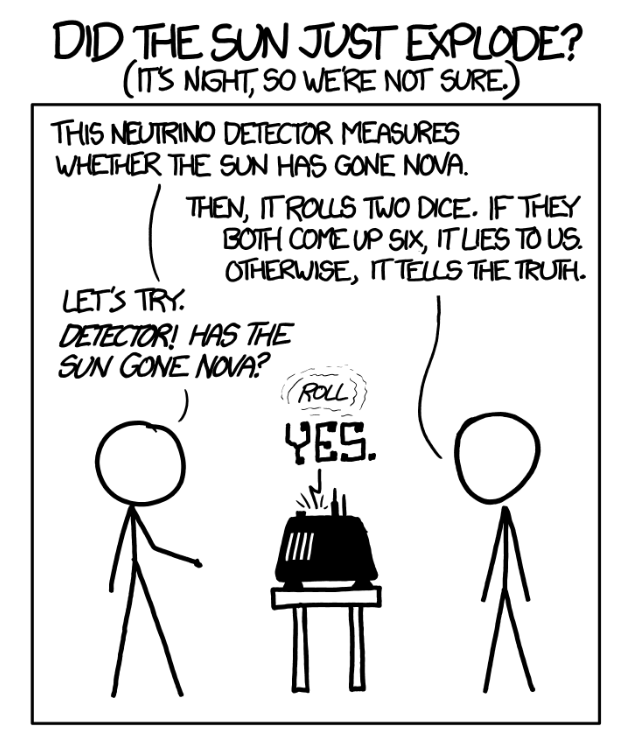
\includegraphics[height=5cm,keepaspectratio]{xkcd}
\end{frame}

\begin{frame}[allowframebreaks]{Frequentism vs Bayesianism} 
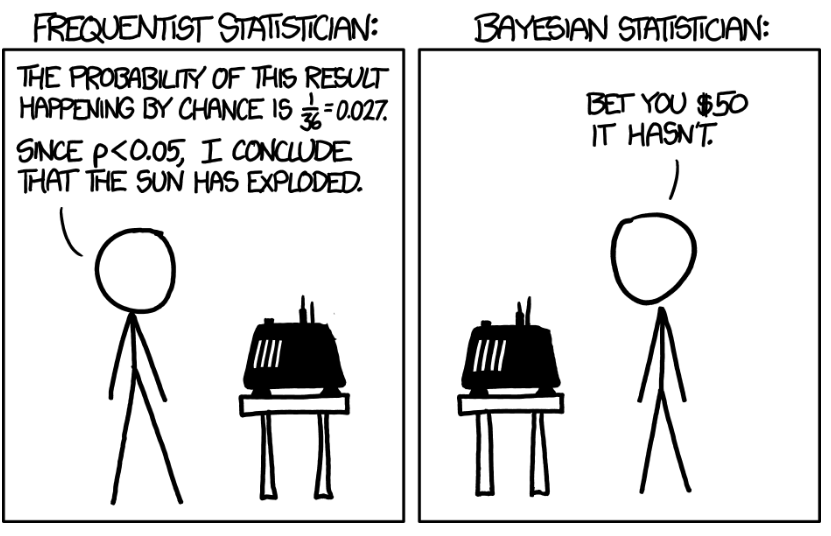
\includegraphics[height=5cm,keepaspectratio]{xkcd2}
\end{frame}

\begin{frame}{Frequentist vs Bayesian} 
빈도주의자들은 확률을 \textbf{특정 사전이 일어날 빈도}로 파악한다. 빈도를 정의하기 위해서는 같은 환경에서의 실험을 반복할 수 있어야 하며, 이러한 반복을 무한히 반복하는 중 나오는 빈도의 극한으로 확률을 정의한다. 즉, 빈도주의자들에게 확률이란 \textbf{어떠한 고정된 값}이며, 동시에 데이터는 랜덤하게 뽑힌 값이다. 

이와는 대조적으로, 베이지안에게는 확률은 어떠한 고정된 값이 아니라, 어떤 \textbf{명제의 확실한 정도를 나타내는 척도}이다. 따라서 확률은 데이터와 사전지식에 의거해서 지식을 수치화하는 하나의 체계이며, \textbf{고정된 값이 아니다.} 대조적으로, 데이터는 관측된 값으로 그것은 고정된 값이다. 
\end{frame}

\begin{frame}[allowframebreaks]{MLE vs MAP}

두 접근의 차이를 알아보기 위해서, 어떤 별의 밝기를 측정하는 실험을 생각해 보겠다. n번의 관측을 통해서 밝기 $F_i$와 에러\footnote{정규분포에서의 표준편차라고 생각해야 한다. 오차-관측값 = 참값이 되는 오차가 아니다. } $e_i$를 안다고 생각하자. 즉, 

\begin{equation}
P(D_i|F = F_t) = \frac{1}{\sqrt{2 \pi e_i^2}}e^{\frac{-(F_i - F_t)^2}{2e_i^2}}
\end{equation}

이다. 이 때, 관측된 $D_i$들에 대해서 다음과 같이 likelihood 함수를 생각할 수 있다. 

\begin{equation} 
L(D|F = F_t) = \Pi P(D_i|F = F_t)
\end{equation} 

이를 최소한으로 만드는 $F_t$를 구하는 것을 \textbf{Maximum Likelihood Estimation}이라고 한다. 

\begin{equation} 
\frac{dL}{dF_t} = 0
\end{equation}

의 근 $F_{estimate}$를 구하고, 이것을 $F_t$로 간주한다. 빈도주의자들에 따르자면 관측한 데이터가 충분히 많으면 이 진술은 참이 되며, 이를 대수의 법칙(Law of Large Numbers)라 한다. 

이것과 대조적으로, 베이지안은 $P(F=F_t|D)$가 최대가 되는 $F_t$를 찾고자 한다. 관측은 우리에게 $P(D|F=F_t)$를 알게 해주므로, 원하는 $F_t$를 구하기 위해서 베이즈의 법칙을 사용한다. 즉, 

\begin{equation} 
P(F = F_t | D) = \frac{P(D|F=F_t)P(F=F_t)}{P(D)}
\end{equation}
이다. 여기서 각 항들의 의미를 살펴보면 

\begin{itemize} 
\item $P(F = F_t | D)$ : Posterior 확률
\item $P( D | F = F_t )$ : Likelihood 
\item $P(F = F_t )$ : Model prior / Prior 확률
\item $P(D)$ : data probability 
\end{itemize} 



\end{frame}

% \begin{frame}{Linear Regression Revisited} 

% \end{frame}

% \begin{frame}[allowframebreaks]{Confidence Interval vs Credible Interval}

% \end{frame}


% \begin{frame}[allowframebreaks]{Example : Estimate on Normal Distribution}

% \end{frame}

% \begin{frame}[allowframebreaks]{Model Selection}

% \end{frame}

% \section{다변수 확률분포}

% \subsection{이산 확률분포} 

% \begin{frame}[allowframebreaks]{Multivariate Discrete Random Variable}

% \end{frame}


% \subsection{연속 확률분포} 

% \begin{frame}[allowframebreaks]{Multivariate Discrete Random Variable}

% \end{frame}


% \subsection{확률분포의 성질들}

% \begin{frame}{Independence}    

% \end{frame}

% \begin{frame}{Expected Value}

% \end{frame}

% \begin{frame}[allowframebreaks]{Properties of Expected Value}

% \end{frame}

% \begin{frame}[allowframebreaks]{Variance, Covariance, and Correlation}

% \end{frame}

% \begin{frame}[allowframebreaks]{Linear Function of Random Variables}

% \end{frame}

% \begin{frame}{Conditional Expectations and Variance}

% \end{frame}

% \begin{frame}{Theorems about Conditional Expectations and Variance}

% \end{frame}


    

% \begin{frame}{Poisson Compounding Equations}

% \end{frame}

% \begin{frame}{Binomial Compounding Equations}

% \end{frame}




% \section{Statistical Inference} 





% \section{Stochastic Process}

% \subsection{Markov Chain} 

% \begin{frame}{Motivation}

% \end{frame}

% \begin{frame}{Markov Chain}

% \end{frame}

% \begin{frame}{Gambler's Ruin Problem}

% \end{frame}


% \begin{frame}{Markov Chain Monte Carlo Methods}

% \end{frame}

% \begin{frame}{Hidden Markov Models}

% \end{frame}



% \subsection{Poisson Process} 

% \begin{frame}{Exponential Distribution}

% \end{frame}

% \begin{frame}{Properties of Exponential Distribution}

% \end{frame}

% \begin{frame}{Convolutions of Exponential Distribution}

% \end{frame}

% \begin{frame}{Poisson Process}

% \end{frame}


% \begin{frame}{Conditional Poisson Process}

% \end{frame}

% \begin{frame}{Software Reliability Estimation}

% \end{frame}



% \subsection{Gaussian Process} 
 
% \subsection{Brownian Motion Process}

% \begin{frame}{Recap on Random Walk}

% \end{frame}


% \begin{frame}{Brownian Motion Process}

% \end{frame}

% \begin{frame}{Stock Price Analysis}

% \end{frame}





\end{document}


